\chapter{Testdurchführungen}
\label{chap:Testphasen}

Es wurden im Rahmen dieser Arbeit eine grosse Anzahl an Messungen und Testfällen durchgeführt. Die Testkonzepte im digitalen Anhang \ref{AnhangDig} geben detailliert Auskunft über die Testdurchführung. Einige Resultate wurden bereits im vorherigen Kapitel eingebunden. Auf den nachfolgenden Seiten werden weitere bedeutsame Resultate wiedergegeben. 

\section{Messinstrumente}

Für die Messungen wurde das Panasonic AMG8834 Eval Kit, welches in Abbildung \ref{fig:grideyeboard} verwendet. Es bietet den Vorteil, dass sich, dank einem Atmel Mikroprozessor und einer bereits vorhandene Software, die Sensordaten als Rohdaten über USB bzw. \ac{UART} mit dem Programm H-Term auslesen lassen. 
Das erstellte C-Programm ConvertValue\_V2\footnote[13]{Im digitalen Anhang bereitgestellt} wandelt die Rohdaten in \ac{CSV}-Files um, damit diese mit Matlab und Python verwendet werden können. Nähere Erläuterungen folgen im Kapitel \ref{chap:Personendetektion}.


\begin{figure}[H]
	\centering
	\includegraphics[width=0.6\linewidth]{fig/grideye_board}
	\caption[Grid Eye Eval Kit]{Grid Eye Eval Kit}
	\label{fig:grideyeboard}
	[\protect\cite{AMG8834}]
\end{figure}



Zudem können die Daten zur Echtzeit über das Bluetooth Modul an die zur Verfügung stehende Grid-Eye App übermittelt werden, damit die aktuellen Werte visualisierbar sind.

Als weitere Messmittel wurden das digitale Thermometer Fluke 52-II und die Wärmebildkamera Fluke TI-125 verwendet, damit Sensorwerte verifiziert werden können. Entsprechende Datenblätter sind im digitalen Anhang \ref{AnhangDig} einsehbar.

\section{Grundlagenmessungen}

Die Grundlagenmessungen geben Auskunft über die Eigenheiten des Messprinzips. Dabei wurden physikalische Aspekte, welche im vorherigen Kapitel erläutert wurden, verifiziert und weitere Erkenntnisse dargelegt. Die nachfolgenden Unterkapitel sind abschnittsweise in Fragestellung, Vorgehen und Ergebnisse gegliedert.

\subsection{Streuung}

\textbf{Fragestellung:} Um eine Person zu detektieren, benötigt es eine Temperaturdifferenz zwischen der Umgebung und der Person. Daher stellt sich die Frage, wie gross die Streuung der Sensorwerte sind. Diese Streuung gibt die minimale Differenz vor, damit eine Person vom Hintergrund unterschieden werden kann.

\textbf{Vorgehen:} In einem 60-minütigen Messdurchgang bei konstanter Umgebungstemperatur von 22.5 °C wurde eine gleichmässig mit 22.6 °C warme Oberfläche ausgemessen. In Abbildung \ref{fig:temperaturverhalten} sind die Thermistorwerte (\textcolor{blue}{blau}) und die 64 Pixelwerte (zwischen \textcolor{red}{rot} \& \textcolor{orange}{orange}) dargestellt.
\begin{figure}[H]
	\centering
	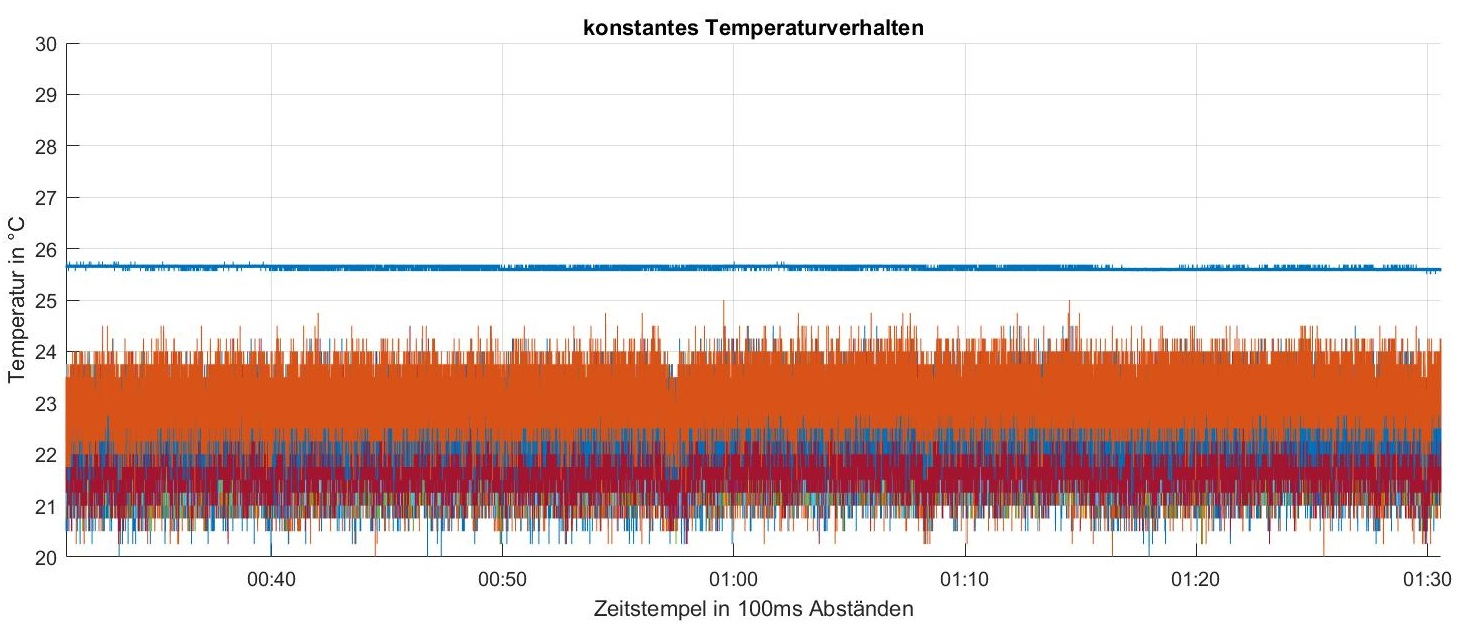
\includegraphics[width=1.0\textwidth]{fig/Temperaturverhalten}
	\caption[Konstantes Temperaturverhalten]{Konstantes Temperaturverhalten}
	\label{fig:temperaturverhalten}
\end{figure}

\textbf{Ergebnisse:} Es fällt auf, dass  der Thermistorwert (\textcolor{blue}{blau}) entgegen den Erwartungen eine höhere Temperatur (25.5 °C anstelle von 22.5 °C) aufweist. Es wurden mehrere Eval Kits ausgetestet und es konnte kein einheitlicher Offset\footnote[14]{Konstanter Versatz von Effektivwert} eruiert werden. Daher ist von Exemplarstreuungen\footnote[15]{Nicht identische Eigenschaften eines Produkts in der Serienherstellung} auszugehen. Die Thermistorwerte sind im Allgemeinen um mehrere Grad höher als die effektiven Werte. 

Zusätzlich ist in der Abbildung \ref{fig:temperaturverhalten} ersichtlich, dass die Temperaturwerte der einzelnen Pixel nicht auf gleichem Niveau liegen. Die Pixelreihe \textcolor{orange}{orange} streut um 23 °C, wobei die Pixelreihe \textcolor{red}{rot} deutlich tiefer liegt. Daher kann nicht davon ausgegangen werden, dass die Sensoren bei einheitlicher Oberflächentemperatur, einheitliche Werte liefern. Die Messabweichung aller 64 Pixel liegt jedoch im Bereich von +/- 1.5 °C vom Mittelwert. 

Diese Messung bietet eine weitere Erkenntnis im Zusammenhang mit der Streuung. Dabei stellte sich heraus, dass die Sensordaten einer Gaussverteilung\footnote[16]{Auch Normalverteilung genannt} folgen. Daher wurde die Standardabweichungen\footnote[17]{Abweichung vom Mittelwert} der einzelnen Pixelwerte ausgewertet. Es wurden anhand nachfolgender Abbildung \ref{fig:Streuung} festgestellt, dass die zentralen Pixel tiefere Abweichungen aufweisen, als die äusseren Pixel.

\begin{figure}[H]
	\centering
	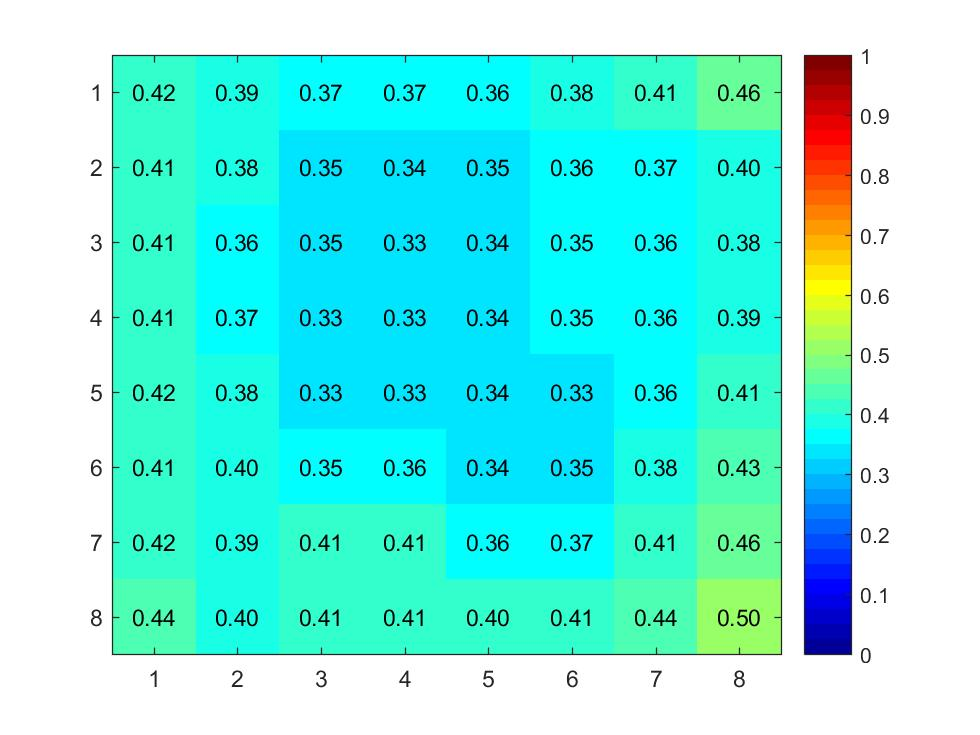
\includegraphics[width=0.5\textwidth]
	{fig/Distanz_140cm_std_.jpg}
	\caption[Standardabweichung der einzelnen Pixel im Vergleich]{Standardabweichung der einzelnen Pixel im Vergleich}
	\label{fig:Streuung}
\end{figure}

Dies könnte in Verbindung mit der konvexen Linse entstehen, da die Sammellinse an den Rändern höhere Beugungs- und Brechungsfehler verursacht. Ein weitere These ist die grössere Messdistanz aufgrund des \ac{FOV} an den Randpunkten. Es muss in jedem Fall mit grösseren Messabweichungen gerechnet werden, wenn sich Personen am Rande des Messbereichs befinden.

\subsection{Einfluss von Lichtquellen}
\textbf{Fragestellung:} Im Unterkapitel \ref{subsec:Personenaufzuege} wurden bereits aus theoretischer Sicht über Einflüsse von Lichtquellen recherchiert. Es stellt sich die Frage, ob übliche Lichtquellen in Aufzügen als Störquellen ausgeschlossen werden können. Daher wird mit dieser Messdurchführung dies verifiziert.

\textbf{Vorgehen:} In mehreren Messdurchläufen wurde der Sensor während 10 Minuten in einem Abstand von 1 Meter auf eine Betonfläche\footnote[18]{Emissionsgrad 0.92 nach Anhang \ref{AnhangE}} gerichtet. Die verwendete Lichtquelle ist unterhalb davon angebracht und wirkt auf dieselbe Fläche. Dabei wurde der Sensor von der Lichtquelle abgeschattet. Die Umgebungstemperatur ist bei allen Durchführungen bei 22 °C +/- 1°C.

\begin{figure}[H]
	\centering
	\includegraphics[width=1.0\textwidth]
	{fig/Lichtquellenvergleich.jpg}
	\caption[Streuung der einzelnen Pixel im Vergleich]{Streuung der einzelnen Pixel im Vergleich}
	\label{fig:Lichtquellen2}
\end{figure}

\textbf{Ergebnisse:}  Wie zu erwarten war, sind die vier Plots in \ref{fig:Lichtquellen2} in gleicher Größenordnung. Bei abgedunkelten Raum, bei Tageslicht und bei einer Leuchtstoffröhre als Beleuchtung gibt es keine nennenswerte Differenzen. Lediglich beim kurzwelligen Infrarot-Wärmestrahler wurden Oberflächen punktuell erwärmt, was zu einer stetigen Zunahme einzelner Pixelwerte führte. 
\newpage
\subsection{Einfluss von  Sonneneinstrahlung}

\textbf{Fragestellung:} Der Sensor ist empfindlich auf Infrarotreflexionen und auf die Temperaturen der Messobjekte\footnote[19]{Siehe Unterkapitel  \ref{sec:Physik}}. Dabei ist die Sonne eine bedeutender Wärmestrahler. Aus diesem Grund wurde im Außenbereich eine Betonoberfläche\footnote[20]{Emissionsgrad 0.92 nach Anhang \ref{AnhangE}} ausgemessen, damit Aussagen über die Sonneneinwirkung gemacht werden können. 

\textbf{Vorgehen:} In einem Messaufbau wurde der Sensor abgeschattet von der Sonne platziert. Dabei ist dieser bei einem Abstand von 1 Meter auf eine Betonfläche gerichtet. Die Betonfläche wurde direkt von der Sonne bestrahlt und wird im Verlauf der Messung abgeschattet. Währendem eine konstante Umgebungstemperatur von 25 °C herrscht.  


\begin{figure}[H]
	\centering
	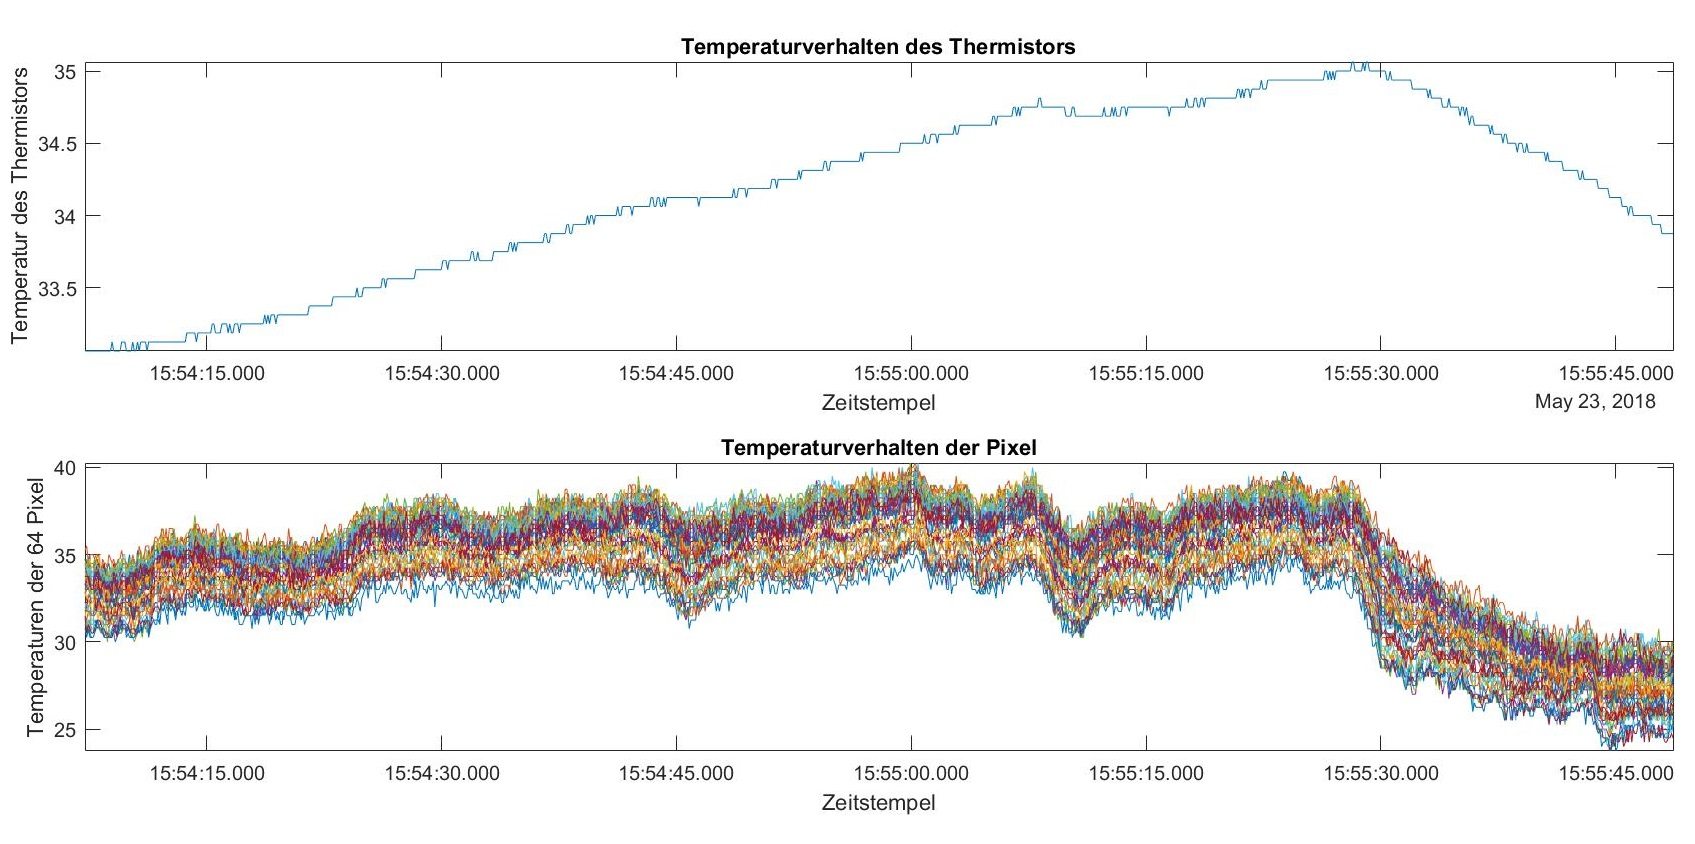
\includegraphics[width=1.0\textwidth]{fig/Temperaturverhalten2}
	\caption[Temperaturverlauf Thermistor/Pixel Messversuch Sonneneinstrahlung]{Temperaturverlauf Thermistor/Pixel Messversuch Sonneneinstrahlung}
	\label{fig:temperaturverhalten2}
\end{figure}

\textbf{Ergebnisse:} In der Abbildung \ref{fig:temperaturverhalten2} sind die Thermistor- und Pixelwerte dargestellt. Einerseits ist ersichtlich, dass bei konstanter Umgebungstemperatur der Thermistorwert weiterhin steigt durch die Wärmestrahlung der Sonne. Dies hat direkten Einfluss auf die Zunahme der Pixelwerte. Im Aussenbereich ist im Allgemeinen eine grössere Differenz zwischen den Pixeln feststellbar.

Kur vor dem Zeitpunkt 15:55:30.000 wird der Messbereich durch eine Holzplatte vom direkten Sonnenlicht abgeschattet. Man erkennt deutlich, dass die Therimstor- und Pixelwerte innerhalb von 15 s bedeutend sinken. Dies hat mit der fehlenden Wärmeeinstrahlung der Sonne zu tun. Daraus kann geschlossen werden, dass Oberflächen, welche direkt von der Sonne bestrahlt werden, stark beeinflusst werden.

\subsection{Einflussfaktor Luftströme}
\textbf{Fragestellung:} Da gerade im Aussenbereich mehr Störquellen für den Sensor vorhanden sind, wurden weitere äussere Einflüsse ausgemessen. Es stellte sich die Frage, ob auch Luftströme Einfluss auf die Messresultate nehmen.

\textbf{Vorgehen:} Ähnlich wie der vorherige Messaufbau wurde der Sensor und der Messbereich abgeschattet von der Sonne platziert. Der Sensor wurde bei einem Abstand von 1 Meter auf eine Betonfläche gerichtet. Die Umgebungstemperatur mass während diesem Messversuch 25.2 °C +/- 0.3 °C.  
	
\begin{figure}[H]
	\centering
	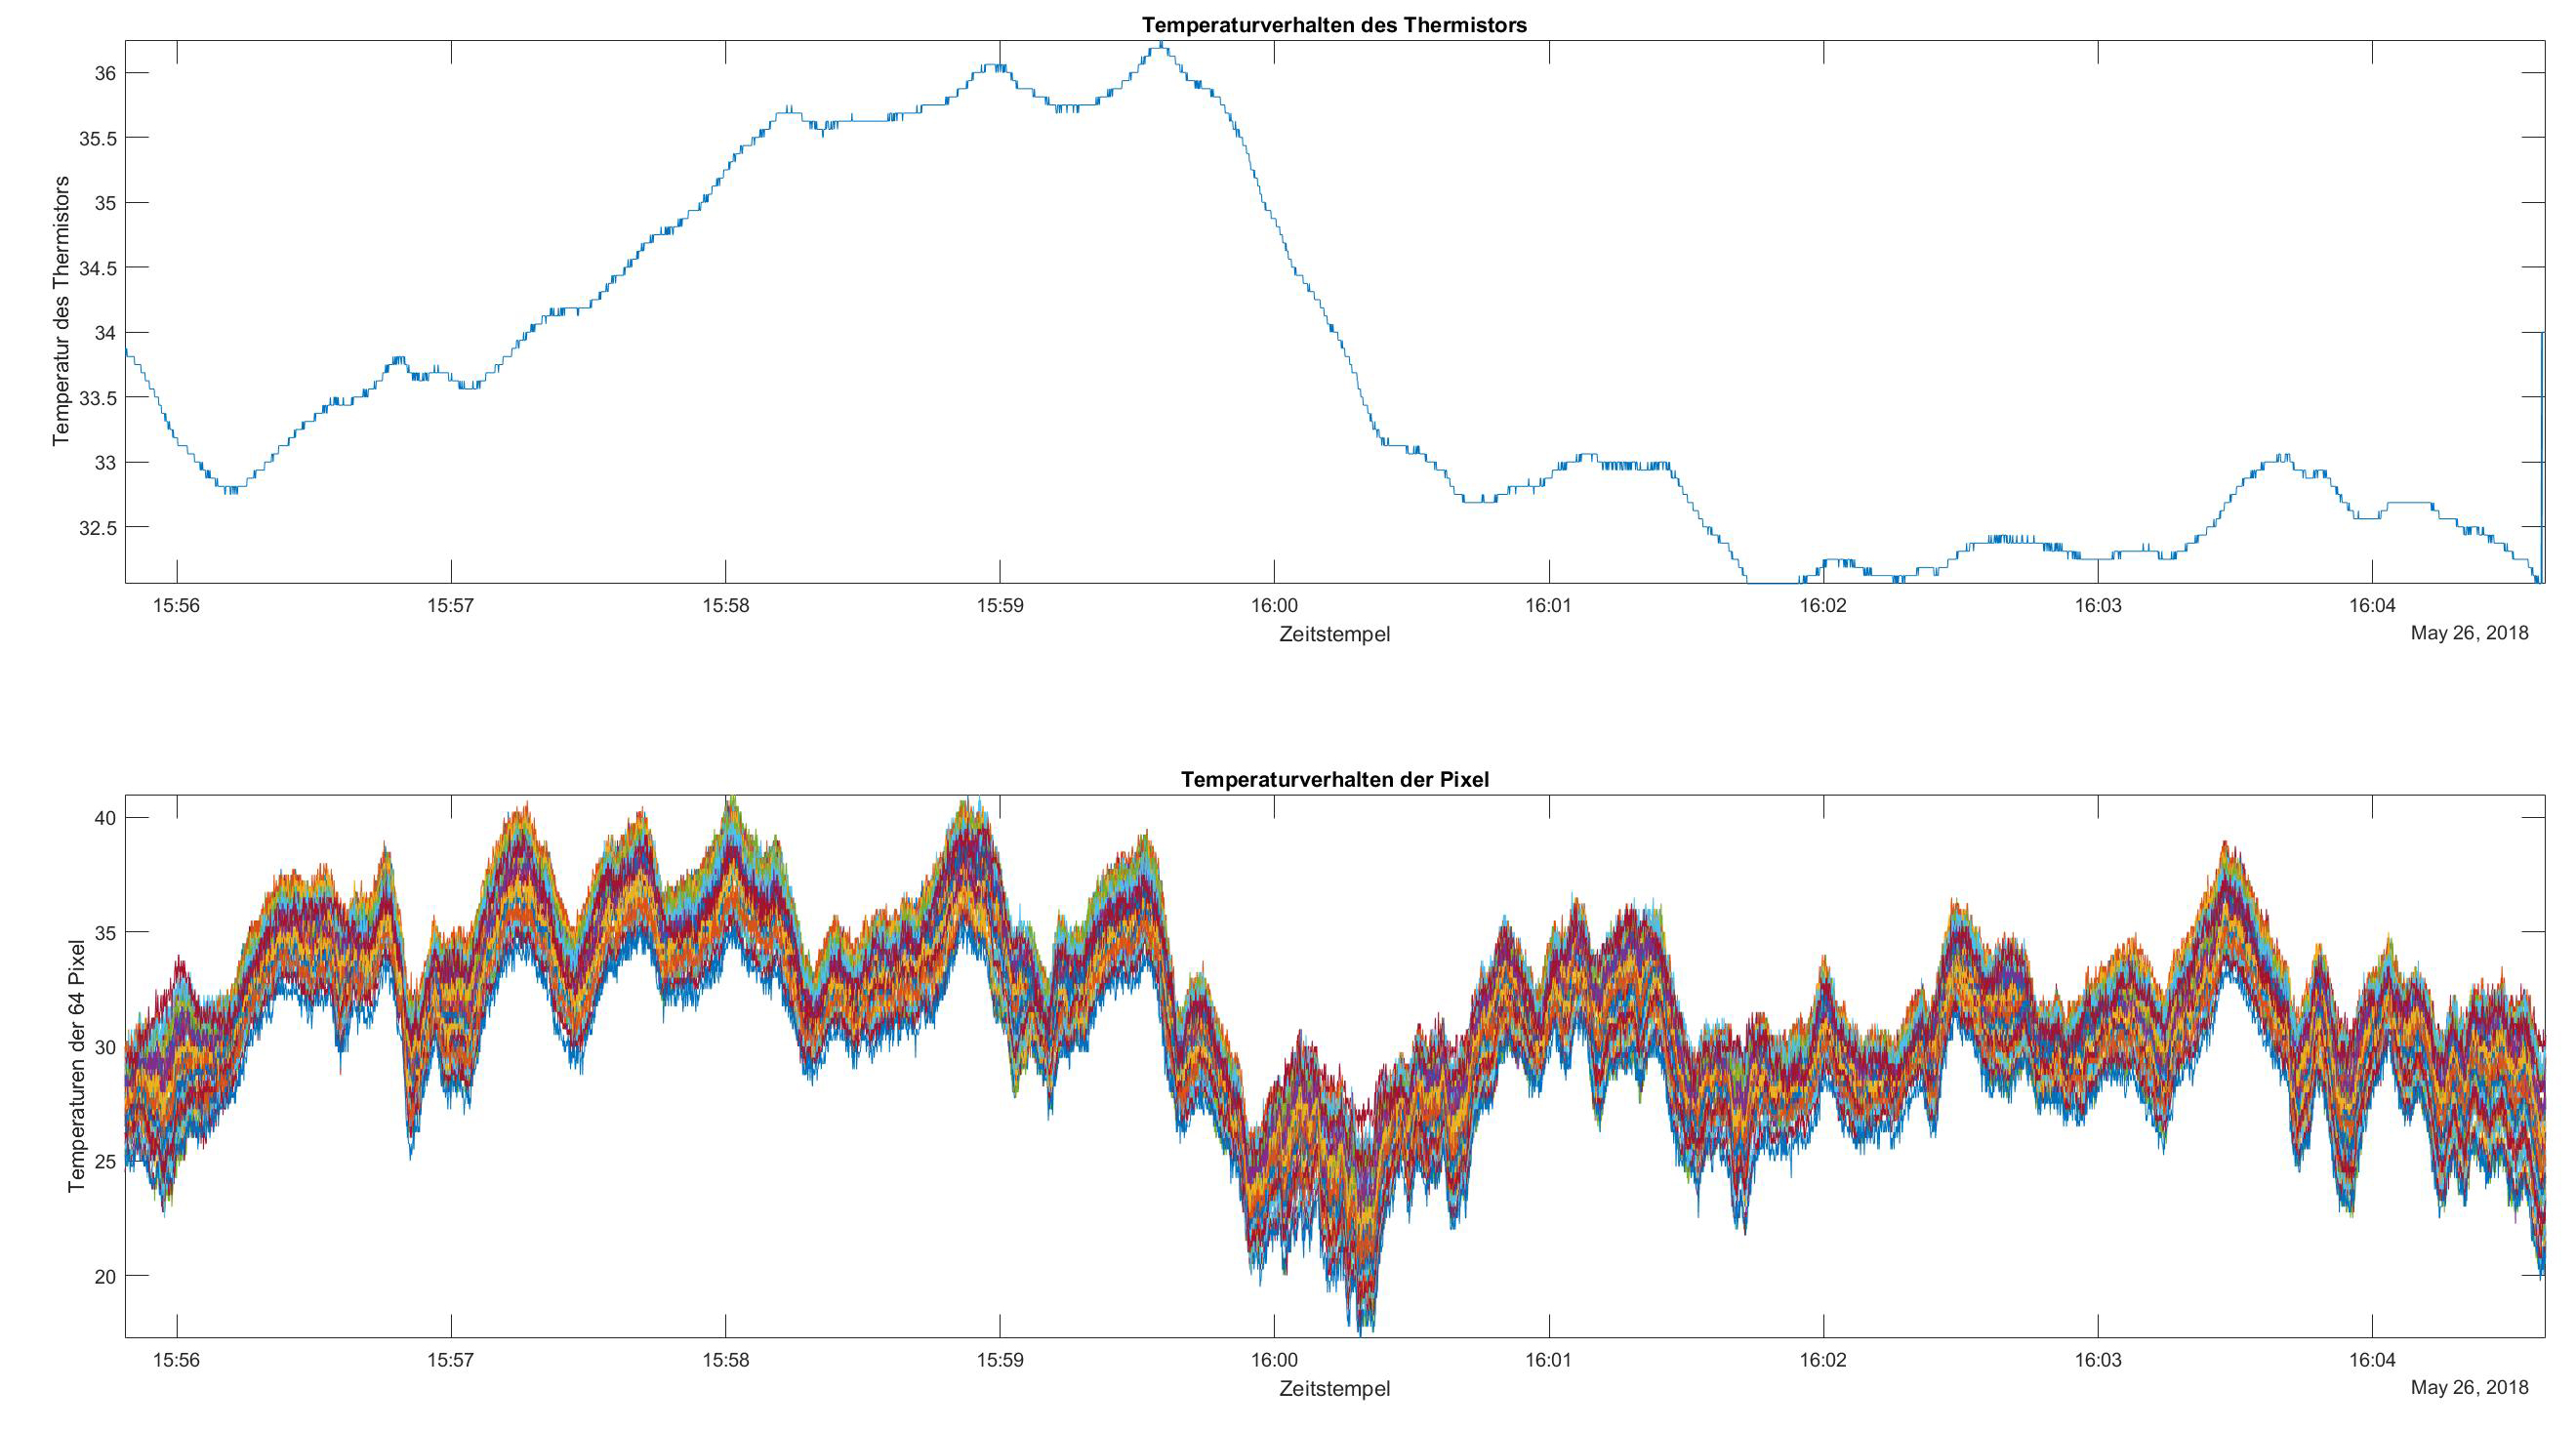
\includegraphics[width=1.0\textwidth]{fig/Temperaturverhaltenwind}
	\caption[Temperaturverlauf Thermistor/Pixel Messversuch Luftströme]{Temperaturverlauf Thermistor/Pixel Messversuch Luftströme}
	\label{fig:temperaturverhaltenwind}
\end{figure}

\textbf{Ergebnisse:} In der Abbildung \ref{fig:temperaturverhaltenwind} sind unregelmäßige Windböen die Ursache für die zum Teil starken Abweichungen der Pixelwerte. Die Spannweite der Pixelwerte erstreckt sich zwischen 40 °C bis 18 °C, wobei die Temperatur lediglich von 36 °C bis 32 °C variiert. Somit besitzen Luftströme, wie beispielsweise Wind Einfluss auf die Messergebnisse. 

\newpage
\section{Personenmessungen}
Bei den Personenmessungen wurden unterschiedliche Probanden in mehreren Aufzügen ausgemessen und auf dessen Wärmestrahlung analysiert. Dabei wurde der Sensor nach Unterkapitel \ref{sec:geometrie} zentral befestigt. Dies ist in Abbildung \ref{fig:img0336} ersichtlich.

\begin{figure}[H]
	\centering
	\includegraphics[width=1.0\linewidth]{fig/IMG_0336}
	\caption[Zentrierte Messeinheit im Aufzug]{Zentrierte Messeinheit im Aufzug}
	\label{fig:img0336}
\end{figure}

\textbf{Fragestellung:} Einerseits soll mit diesen Messungen geklärt werden, wie sich mehrere Personen im Messbereich auf den Sensor auswirken und anderseits dienen diese Messdaten gleichzeitig als Datensätze für weitere Untersuchungen.

\textbf{Vorgehen:} Es standen insgesamt sechs Probanden zur Verfügung. Die Probanden wurden entsprechend ihrer Grösse und dem Körperumfang in die Kategorien klein [K], mittel [N] und gross [G] unterteilt. Die Tabelle \ref{tab:probanden} gibt Auskunft über die Masse der Probanden. Dabei handelt es sich durchgehend um die grössten Werte. 

\begin{table}[H]
	\centering
	\caption[Masse der Probanden in {[cm]} ]{Masse der Probanden in [cm]}
	\label{tab:probanden}
	\begin{tabular}{|
			>{\columncolor[HTML]{C0C0C0}}c |c|c|c|c|}
		\hline
		& \cellcolor[HTML]{C0C0C0}\textbf{  Grösse  } & \cellcolor[HTML]{C0C0C0}{\color[HTML]{333333} \textbf{  Breite }} & \cellcolor[HTML]{C0C0C0}{\color[HTML]{333333} \textbf{  Tiefe }} & \cellcolor[HTML]{C0C0C0}\textbf{Kategorie} \\ \hline
		\textbf{Proband 1} & 162                                              & 46                                                                      & 28                                                                     & k                                          \\ \hline
		\textbf{Proband 2} & 166                                              & 52                                                                      & 33                                                                     & k                                          \\ \hline
		\textbf{Proband 3} & 167                                              & 48                                                                      & 25                                                                     & k                                          \\ \hline
		\textbf{Proband 4} & 172                                              & 53                                                                      & 34                                                                     & m                                          \\ \hline
		\textbf{Proband 5} & 175.5                                            & 54                                                                      & 34                                                                     & m                                          \\ \hline
		\textbf{Proband 6} & 185.5                                            & 63.5                                                                    & 42                                                                     & g                                          \\ \hline
	\end{tabular}
\end{table}

\newpage
Für den Messaufbau wurde ein Raster erstellt, welches einerseits den gesamten \ac{FOV} des Sensors abdeckt und anderseits in unterschiedlich grossen Personenaufzügen anwendbar ist. Aus dem Größenvergleich von üblichen Personenaufzügen wurde ein gemittelte Grösse berechnet. Die berechnete Masse sowie der Aufbau des Rasters ist in der Abbildung \ref{fig:Messraster} dargestellt.
 
\begin{figure}[H]
	\centering
	\includegraphics[width=1.0\textwidth, angle=0]{fig/Messraster_bearbeitet.JPG}
	\caption[Messraster für Personenmessungen]{Messraster für Personenmessungen}
	\label{fig:Messraster}
\end{figure}

Die Abstände der 12 Messpunkte A - L sind, so berechnet, dass Personen nebeneinander stehen können. Es können dadurch unterschiedliche Variationen an Personenmessungen durchgeführt werden, indem die Probanden an den Punkten platziert werden. Im Anhang \ref{AnhangD} sind die verschieden Aufzüge abgebildet und parametrisiert.

\newpage

\textbf{Ergebnisse:} Insgesamt wurden pro Aufzug 50 unterschiedliche Messungen\footnote[21]{Messdaten im digitalen Anhang angefügt} durchgeführt. Dabei wurden auf eine unterschiedliche Anzahl an Personen und auf verschiedene Probandengrössen geachtet. Es handelt sich dabei um je einminütige ,stationäre Aufnahmen, welche jede circa 600 Frames\footnote[22]{Einzelbild einer Bildsequenz} bieten. In Abbildung \ref{fig:p1gallpositionsmean} sind sechs Medianwerte der 1-Personenmessungen ersichtlich. In der oberen Reihe wurde ein Proband der Kategorie G eingesetzt. In der unteren Reihe wurde ein Proband der Kategorie K verwendet. Es ist ersichtlich, dass die Personenprofile stark abweichen, da sich die Distanz zum Sensor aufgrund der Körpergrösse unterscheiden.

\begin{figure}[H]
	\centering
	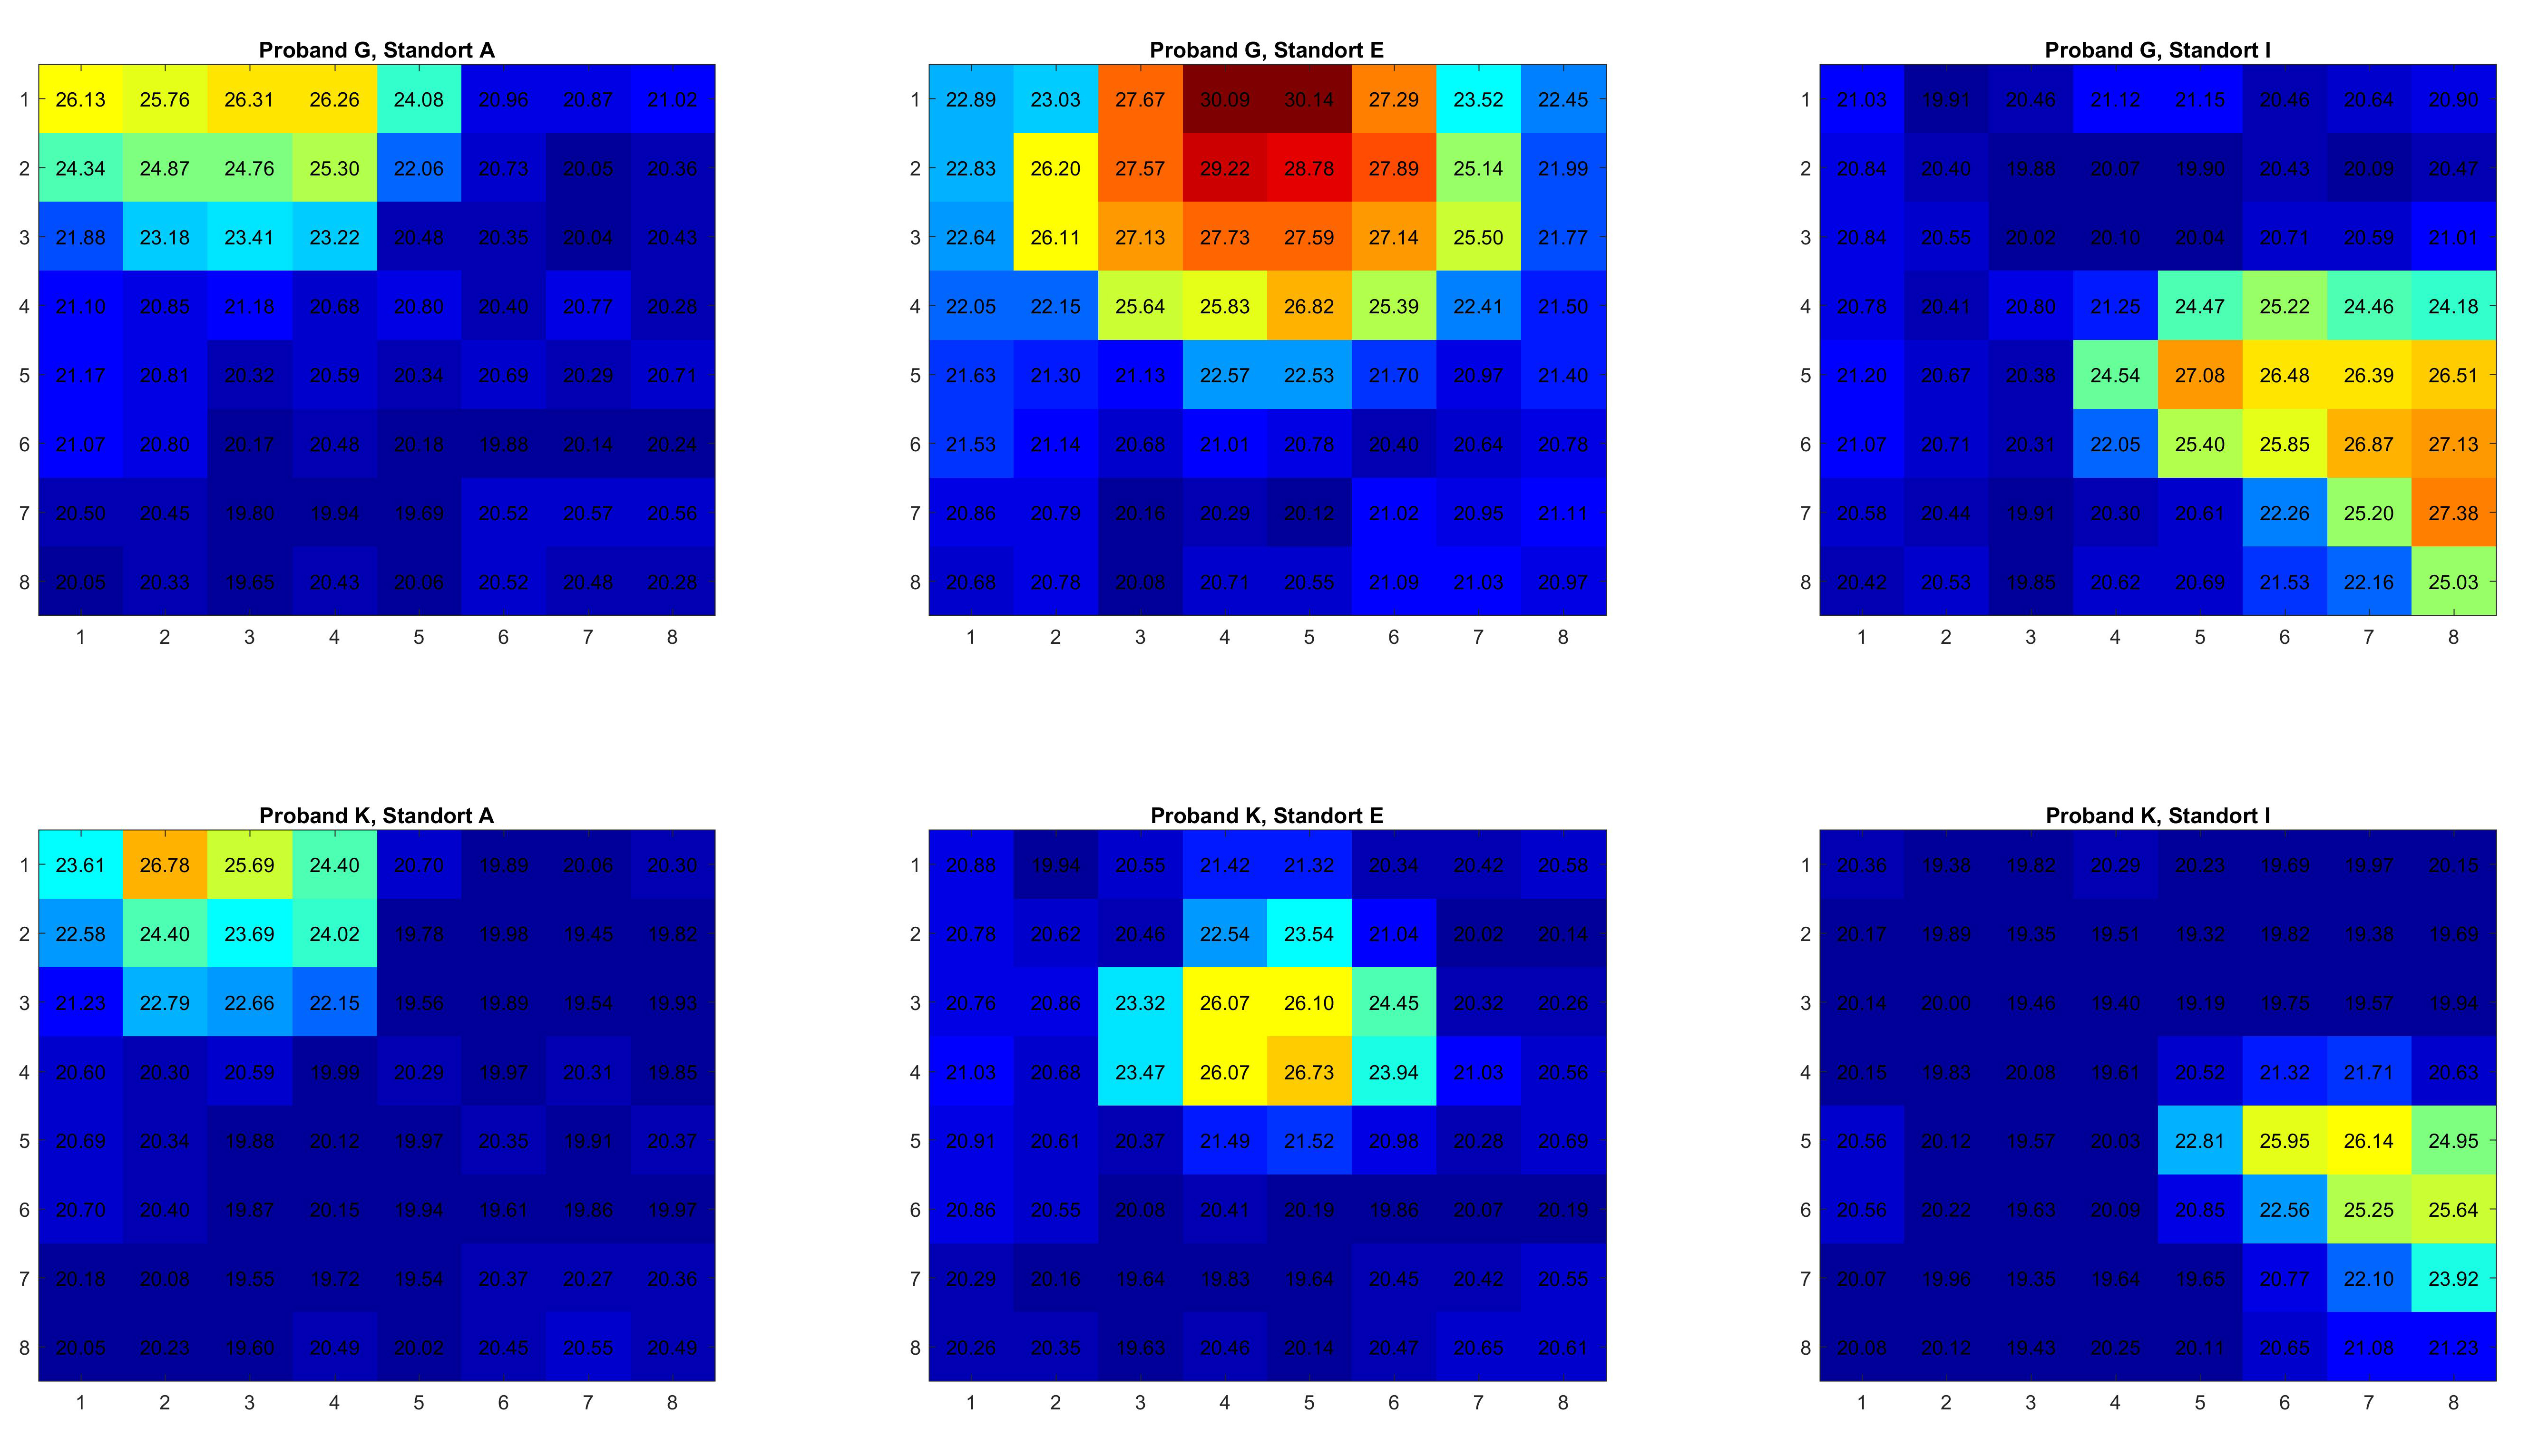
\includegraphics[width=1.0\textwidth]{fig/p1_k_g_aei.jpg}
	\caption[Medianwerte Messung V1 Kategorie G]{Medianwerte Messung V1 Kategorie G}
	\label{fig:p1gallpositionsmean}
\end{figure}

Zudem sind freie Hautoberflächen wie der Kopf, zu sehen beispielsweise beim Proband G am Standort E, bedeutend wärmer. An den Rändern des Messbereichs wir aufgrund der Perspektive die Person nicht von oben ausgemessen, sondern seitlich. Dies führt dazu, falls der Kopf ausserhalb des Messbereichs liegt, dass die Messwerte deutlich tiefer liegen. Für die Personenerkennung ist diese Situation schwieriger zu identifizieren.

Messungen mit ein bis zwei Personen werden, sofern sie sich nicht unmittelbar nebeneinander befinden, gut separiert. 
Aufgrund der begrenzten Auflösung ist die Erkennung bei drei und vier Personen deutlich schwieriger. In Abbildung \ref{fig:p33x3allpositons} sind vier Messungen dargelegt, welche mit je einem Proband der Kategorie G, K und M durchgeführt wurden.

\begin{figure}[H]
	\centering
	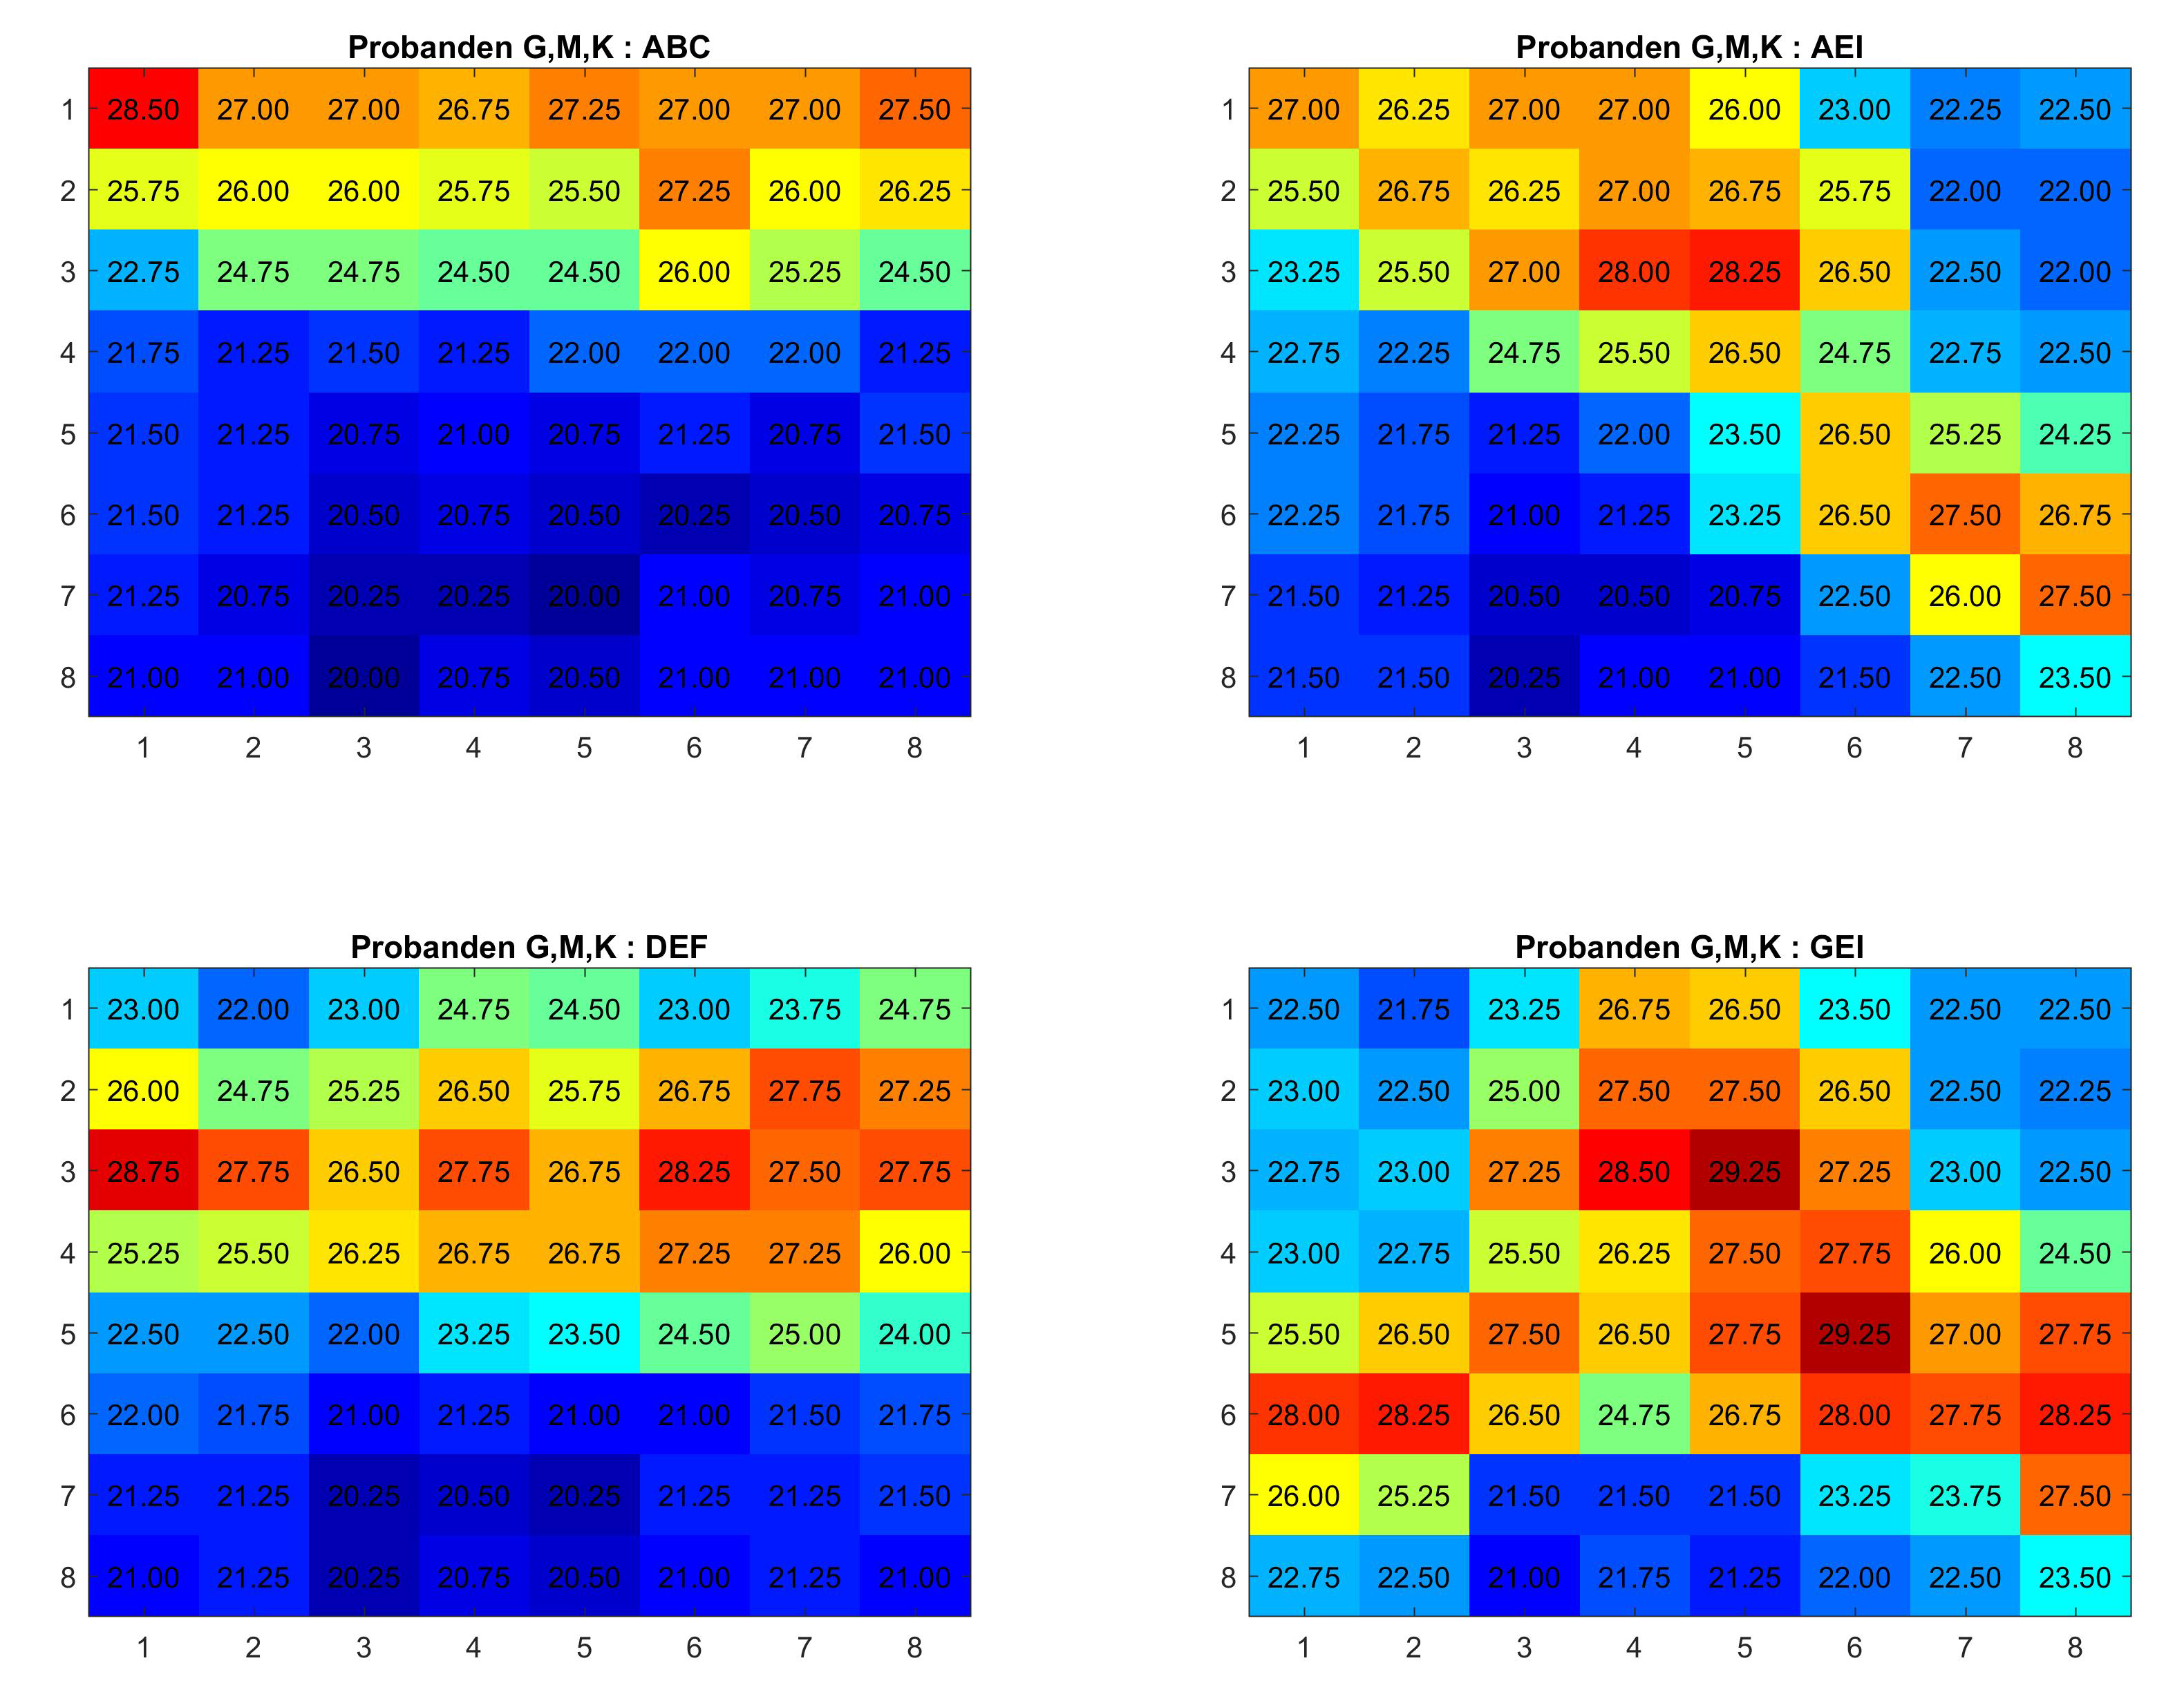
\includegraphics[width=0.8\linewidth]{fig/p3_kkg_4x4.jpg}
	\caption[Medianwerte aus Messungen mit 3 Personen der Kategorie: GMK]{Medianwerte Messungen 3 Personen Kategorie: GMK}
	\label{fig:p33x3allpositons}
\end{figure}


Bei Abbildung DEF und GEI können die drei Probanden durch ihren Kopf, als wärmstes Zentrum, voneinander differenziert werden. Bei den Randregionen ABC ist dies deutlich schwieriger. Die Schwierigkeit liegt darin, bei naheliegenden Personen zu differenzieren, ob es sich um mehrere kleinere Personen oder um eine grosse Person handelt.


\section{Fazit}
Die Messresultate haben die Ergebnisse aus dem Kapitel \ref{chap:Informationsbeschaffung} bestätigt. Zudem konnten noch weitere Einflüsse und Störquellen identifiziert werden. Vor allem im Aussenbereich gibt es Störeinwirkungen, die Verfehlungen bei den Sensorwerten verursachen. Es liegt nahe, dieses Messprinzip nicht im Aussenbereichen zu verwenden.
Bei Personenmessungen liegt die Schwierigkeit darin, die individuellen Profile der Personen zu erkennen. Die Grösse der Personen mit der begrenzten Auflösung besitzt nur eingeschränkte Aussagekraft über das Profil. Nahe stehende Personen können leicht um eine Person verwechselt werden. Hinzu kommt die Schwierigkeit, dass die einzelnen Pixel bis zu 2.5 °C streuen. 

Die Messdaten bieten jedoch durch die Streuung der Messwerte auch mehr unterschiedliche Frames. Dies ist vorteilhaft für das neuronale Netzwerk, da die Messungen mehr einzigartige Frames zur Verfügung stellen.